%-----------------------------------------------------------------------------%
\chapter{\babEmpat}
%-----------------------------------------------------------------------------%

%-----------------------------------------------------------------------------%
\section{Petunjuk Penggunaan}
%-----------------------------------------------------------------------------%

\textit{Template} tugas akhir ini dibuat menggunakan \latex. Oleh karena itu, dibutuhkan \latex~\textit{builder} untuk mengolah kode yang sudah dibuat. Hasil dari proses \textit{build} adalah \textit{file} PDF (\textit{portable document format}), bukan \textit{.odt} maupun \textit{.doc}. Sehingga dibutuhkan aplikasi PDF \textit{reader} untuk membuka pdf hasil pengolahan kode yang dibuat. Beberapa kode-kode yang dapat digunakan di dalam \textit{template} ini sudah ditunjukkan pada bab3 sesuai dengan contohnya masing-masing.

Lankah paling awal untuk menggunakan \textit{template} ini adalah memodifikasi \textit{konfigurasi.tex}. Modifikasi ini dilakukan dengan merubah nilai-nilai variabel yang terdapat di dalam berkas \textit{konfigurasi.tex}, sehingga nilainya sesuai dengan yang penulis inginkan. Nilai variabel-variabel yang diganti tersebut akan merubah isi berkas pdf, setelah kode-kode tersebut diproses. Untuk memproses \textit{template} ini, penulis hanya perlu men-\textit{build} \textit{main.tex}. Berkas-berkas \textit{.tex} lain akan secara otomatis ter-\textit{build}~juga ketika \textit{main.tex} di-\textit{build}.

Selanjutnya penulis dapat memulai proses penulisan atau pengisian buku. Berkas-berkas yang perlu dirubah antara lain \textit{abstrak.tex, abstract.tex}~berisi abstrak berbahasa Inggris dan Indonesia, \textit{pengantar.tex} berisi kata pengantar, \textit{bab1.tex} hingga \textit{bab5.tex} diisi sesuai yang penulis inginkan, serta \textit{pustaka.tex} untuk memasukkan daftar pustaka.

\begin{figure}
	\centering
	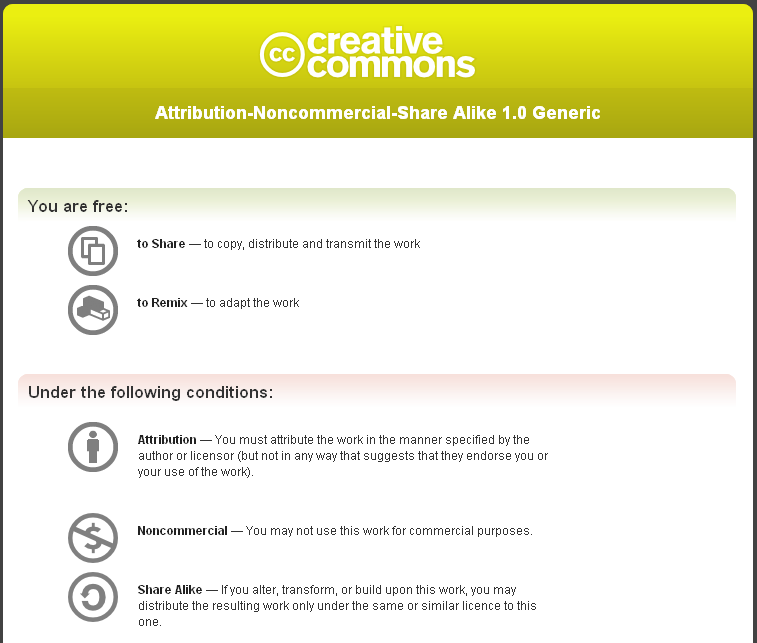
\includegraphics[width=0.3\textwidth]
		{pics/creative_common.png}
		\caption{CC-A-NC-SA 1.0 Generic}
	\label{fig:CC10}
\end{figure}

\textit{Template} tugas ini dipasangkan lisensi \textit{Creative Common---Attribution---Non Commercial---Share Alike 1.0 Generic}.